\documentclass[twoside]{book}

% Packages required by doxygen
\usepackage{fixltx2e}
\usepackage{calc}
\usepackage{doxygen}
\usepackage[export]{adjustbox} % also loads graphicx
\usepackage{graphicx}
\usepackage[utf8]{inputenc}
\usepackage{makeidx}
\usepackage{multicol}
\usepackage{multirow}
\PassOptionsToPackage{warn}{textcomp}
\usepackage{textcomp}
\usepackage[nointegrals]{wasysym}
\usepackage[table]{xcolor}

% Font selection
\usepackage[T1]{fontenc}
\usepackage[scaled=.90]{helvet}
\usepackage{courier}
\usepackage{amssymb}
\usepackage{sectsty}
\renewcommand{\familydefault}{\sfdefault}
\allsectionsfont{%
  \fontseries{bc}\selectfont%
  \color{darkgray}%
}
\renewcommand{\DoxyLabelFont}{%
  \fontseries{bc}\selectfont%
  \color{darkgray}%
}
\newcommand{\+}{\discretionary{\mbox{\scriptsize$\hookleftarrow$}}{}{}}

% Page & text layout
\usepackage{geometry}
\geometry{%
  a4paper,%
  top=2.5cm,%
  bottom=2.5cm,%
  left=2.5cm,%
  right=2.5cm%
}
\tolerance=750
\hfuzz=15pt
\hbadness=750
\setlength{\emergencystretch}{15pt}
\setlength{\parindent}{0cm}
\setlength{\parskip}{3ex plus 2ex minus 2ex}
\makeatletter
\renewcommand{\paragraph}{%
  \@startsection{paragraph}{4}{0ex}{-1.0ex}{1.0ex}{%
    \normalfont\normalsize\bfseries\SS@parafont%
  }%
}
\renewcommand{\subparagraph}{%
  \@startsection{subparagraph}{5}{0ex}{-1.0ex}{1.0ex}{%
    \normalfont\normalsize\bfseries\SS@subparafont%
  }%
}
\makeatother

% Headers & footers
\usepackage{fancyhdr}
\pagestyle{fancyplain}
\fancyhead[LE]{\fancyplain{}{\bfseries\thepage}}
\fancyhead[CE]{\fancyplain{}{}}
\fancyhead[RE]{\fancyplain{}{\bfseries\leftmark}}
\fancyhead[LO]{\fancyplain{}{\bfseries\rightmark}}
\fancyhead[CO]{\fancyplain{}{}}
\fancyhead[RO]{\fancyplain{}{\bfseries\thepage}}
\fancyfoot[LE]{\fancyplain{}{}}
\fancyfoot[CE]{\fancyplain{}{}}
\fancyfoot[RE]{\fancyplain{}{\bfseries\scriptsize Generated by Doxygen }}
\fancyfoot[LO]{\fancyplain{}{\bfseries\scriptsize Generated by Doxygen }}
\fancyfoot[CO]{\fancyplain{}{}}
\fancyfoot[RO]{\fancyplain{}{}}
\renewcommand{\footrulewidth}{0.4pt}
\renewcommand{\chaptermark}[1]{%
  \markboth{#1}{}%
}
\renewcommand{\sectionmark}[1]{%
  \markright{\thesection\ #1}%
}

% Indices & bibliography
\usepackage{natbib}
\usepackage[titles]{tocloft}
\setcounter{tocdepth}{3}
\setcounter{secnumdepth}{5}
\makeindex

% Hyperlinks (required, but should be loaded last)
\usepackage{ifpdf}
\ifpdf
  \usepackage[pdftex,pagebackref=true]{hyperref}
\else
  \usepackage[ps2pdf,pagebackref=true]{hyperref}
\fi
\hypersetup{%
  colorlinks=true,%
  linkcolor=blue,%
  citecolor=blue,%
  unicode%
}

% Custom commands
\newcommand{\clearemptydoublepage}{%
  \newpage{\pagestyle{empty}\cleardoublepage}%
}

\usepackage{caption}
\captionsetup{labelsep=space,justification=centering,font={bf},singlelinecheck=off,skip=4pt,position=top}

%===== C O N T E N T S =====

\begin{document}

% Titlepage & ToC
\hypersetup{pageanchor=false,
             bookmarksnumbered=true,
             pdfencoding=unicode
            }
\pagenumbering{alph}
\begin{titlepage}
\vspace*{7cm}
\begin{center}%
{\Large Documentation Lab\+\_\+1 Delegats }\\
\vspace*{1cm}
{\large Generated by Doxygen 1.8.12}\\
\end{center}
\end{titlepage}
\clearemptydoublepage
\pagenumbering{roman}
\tableofcontents
\clearemptydoublepage
\pagenumbering{arabic}
\hypersetup{pageanchor=true}

%--- Begin generated contents ---
\chapter{Namespace Index}
\section{Packages}
Here are the packages with brief descriptions (if available)\+:\begin{DoxyCompactList}
\item\contentsline{section}{\hyperlink{namespace_c_sharp_lab__1}{C\+Sharp\+Lab\+\_\+1} }{\pageref{namespace_c_sharp_lab__1}}{}
\end{DoxyCompactList}

\chapter{Class Index}
\section{Class List}
Here are the classes, structs, unions and interfaces with brief descriptions\+:\begin{DoxyCompactList}
\item\contentsline{section}{\hyperlink{class_candidate}{Candidate} }{\pageref{class_candidate}}{}
\item\contentsline{section}{\hyperlink{class_error}{Error} }{\pageref{class_error}}{}
\item\contentsline{section}{\hyperlink{class_hr__manager}{Hr\+\_\+manager} }{\pageref{class_hr__manager}}{}
\item\contentsline{section}{\hyperlink{class_interview}{Interview} }{\pageref{class_interview}}{}
\item\contentsline{section}{\hyperlink{class_it__company}{It\+\_\+company} }{\pageref{class_it__company}}{}
\item\contentsline{section}{\hyperlink{class_resume}{Resume} }{\pageref{class_resume}}{}
\item\contentsline{section}{\hyperlink{class_technical__manager}{Technical\+\_\+manager} }{\pageref{class_technical__manager}}{}
\item\contentsline{section}{\hyperlink{class_test}{Test} }{\pageref{class_test}}{}
\item\contentsline{section}{\hyperlink{class_worker}{Worker} }{\pageref{class_worker}}{}
\end{DoxyCompactList}

\chapter{Namespace Documentation}
\hypertarget{namespace_c_sharp_lab__1}{}\section{C\+Sharp\+Lab\+\_\+1 Namespace Reference}
\label{namespace_c_sharp_lab__1}\index{C\+Sharp\+Lab\+\_\+1@{C\+Sharp\+Lab\+\_\+1}}
\subsection*{Classes}
\begin{DoxyCompactItemize}
\item 
class \hyperlink{class_c_sharp_lab__1_1_1_explorer}{Explorer}
\begin{DoxyCompactList}\small\item\em Клас, що відслідковує зміни на матеріально-\/технічній базі \end{DoxyCompactList}\item 
class \hyperlink{class_c_sharp_lab__1_1_1_m_t_b}{M\+TB}
\begin{DoxyCompactList}\small\item\em Клас матеріально-\/технічної бази \end{DoxyCompactList}\item 
class \hyperlink{class_c_sharp_lab__1_1_1_program}{Program}
\end{DoxyCompactItemize}

\chapter{Class Documentation}
\hypertarget{class_c_sharp_lab__1_1_1_explorer}{}\section{C\+Sharp\+Lab\+\_\+1.\+Explorer Class Reference}
\label{class_c_sharp_lab__1_1_1_explorer}\index{C\+Sharp\+Lab\+\_\+1.\+Explorer@{C\+Sharp\+Lab\+\_\+1.\+Explorer}}


Клас, що відслідковує зміни на матеріально-\/технічній базі  


\subsection*{Public Member Functions}
\begin{DoxyCompactItemize}
\item 
\hyperlink{class_c_sharp_lab__1_1_1_explorer_a64fd7698367e71057067ce32a6c47d67}{Explorer} ()
\begin{DoxyCompactList}\small\item\em Конструктор за замовчуванням \end{DoxyCompactList}\item 
int \hyperlink{class_c_sharp_lab__1_1_1_explorer_a42cbc06f2e5c5614bea708dbc43250a6}{Get\+Changes} ()
\begin{DoxyCompactList}\small\item\em гетер \end{DoxyCompactList}\item 
void \hyperlink{class_c_sharp_lab__1_1_1_explorer_a4b685e3fdc095b24a2854f23a44e439b}{Change\+Bought} ()
\begin{DoxyCompactList}\small\item\em Обробка події покупки \end{DoxyCompactList}\item 
void \hyperlink{class_c_sharp_lab__1_1_1_explorer_a65669ed2aaf2eb10382e4644dec50391}{Change\+Brouken} ()
\begin{DoxyCompactList}\small\item\em Обробка події поломки \end{DoxyCompactList}\item 
void \hyperlink{class_c_sharp_lab__1_1_1_explorer_a8f1c353e08ae3448ea231da558b048d9}{Change\+Amortize} ()
\begin{DoxyCompactList}\small\item\em Обробка події списання \end{DoxyCompactList}\end{DoxyCompactItemize}


\subsection{Detailed Description}
Клас, що відслідковує зміни на матеріально-\/технічній базі 



\subsection{Constructor \& Destructor Documentation}
\hypertarget{class_c_sharp_lab__1_1_1_explorer_a64fd7698367e71057067ce32a6c47d67}{}\label{class_c_sharp_lab__1_1_1_explorer_a64fd7698367e71057067ce32a6c47d67} 
\index{C\+Sharp\+Lab\+\_\+1\+::\+Explorer@{C\+Sharp\+Lab\+\_\+1\+::\+Explorer}!Explorer@{Explorer}}
\index{Explorer@{Explorer}!C\+Sharp\+Lab\+\_\+1\+::\+Explorer@{C\+Sharp\+Lab\+\_\+1\+::\+Explorer}}
\subsubsection{\texorpdfstring{Explorer()}{Explorer()}}
{\footnotesize\ttfamily C\+Sharp\+Lab\+\_\+1.\+Explorer.\+Explorer (\begin{DoxyParamCaption}{ }\end{DoxyParamCaption})}



Конструктор за замовчуванням 



\subsection{Member Function Documentation}
\hypertarget{class_c_sharp_lab__1_1_1_explorer_a8f1c353e08ae3448ea231da558b048d9}{}\label{class_c_sharp_lab__1_1_1_explorer_a8f1c353e08ae3448ea231da558b048d9} 
\index{C\+Sharp\+Lab\+\_\+1\+::\+Explorer@{C\+Sharp\+Lab\+\_\+1\+::\+Explorer}!Change\+Amortize@{Change\+Amortize}}
\index{Change\+Amortize@{Change\+Amortize}!C\+Sharp\+Lab\+\_\+1\+::\+Explorer@{C\+Sharp\+Lab\+\_\+1\+::\+Explorer}}
\subsubsection{\texorpdfstring{Change\+Amortize()}{ChangeAmortize()}}
{\footnotesize\ttfamily void C\+Sharp\+Lab\+\_\+1.\+Explorer.\+Change\+Amortize (\begin{DoxyParamCaption}{ }\end{DoxyParamCaption})}



Обробка події списання 

\hypertarget{class_c_sharp_lab__1_1_1_explorer_a4b685e3fdc095b24a2854f23a44e439b}{}\label{class_c_sharp_lab__1_1_1_explorer_a4b685e3fdc095b24a2854f23a44e439b} 
\index{C\+Sharp\+Lab\+\_\+1\+::\+Explorer@{C\+Sharp\+Lab\+\_\+1\+::\+Explorer}!Change\+Bought@{Change\+Bought}}
\index{Change\+Bought@{Change\+Bought}!C\+Sharp\+Lab\+\_\+1\+::\+Explorer@{C\+Sharp\+Lab\+\_\+1\+::\+Explorer}}
\subsubsection{\texorpdfstring{Change\+Bought()}{ChangeBought()}}
{\footnotesize\ttfamily void C\+Sharp\+Lab\+\_\+1.\+Explorer.\+Change\+Bought (\begin{DoxyParamCaption}{ }\end{DoxyParamCaption})}



Обробка події покупки 

\hypertarget{class_c_sharp_lab__1_1_1_explorer_a65669ed2aaf2eb10382e4644dec50391}{}\label{class_c_sharp_lab__1_1_1_explorer_a65669ed2aaf2eb10382e4644dec50391} 
\index{C\+Sharp\+Lab\+\_\+1\+::\+Explorer@{C\+Sharp\+Lab\+\_\+1\+::\+Explorer}!Change\+Brouken@{Change\+Brouken}}
\index{Change\+Brouken@{Change\+Brouken}!C\+Sharp\+Lab\+\_\+1\+::\+Explorer@{C\+Sharp\+Lab\+\_\+1\+::\+Explorer}}
\subsubsection{\texorpdfstring{Change\+Brouken()}{ChangeBrouken()}}
{\footnotesize\ttfamily void C\+Sharp\+Lab\+\_\+1.\+Explorer.\+Change\+Brouken (\begin{DoxyParamCaption}{ }\end{DoxyParamCaption})}



Обробка події поломки 

\hypertarget{class_c_sharp_lab__1_1_1_explorer_a42cbc06f2e5c5614bea708dbc43250a6}{}\label{class_c_sharp_lab__1_1_1_explorer_a42cbc06f2e5c5614bea708dbc43250a6} 
\index{C\+Sharp\+Lab\+\_\+1\+::\+Explorer@{C\+Sharp\+Lab\+\_\+1\+::\+Explorer}!Get\+Changes@{Get\+Changes}}
\index{Get\+Changes@{Get\+Changes}!C\+Sharp\+Lab\+\_\+1\+::\+Explorer@{C\+Sharp\+Lab\+\_\+1\+::\+Explorer}}
\subsubsection{\texorpdfstring{Get\+Changes()}{GetChanges()}}
{\footnotesize\ttfamily int C\+Sharp\+Lab\+\_\+1.\+Explorer.\+Get\+Changes (\begin{DoxyParamCaption}{ }\end{DoxyParamCaption})}



гетер 

\begin{DoxyReturn}{Returns}
Кількість змін
\end{DoxyReturn}


The documentation for this class was generated from the following file\+:\begin{DoxyCompactItemize}
\item 
Explorer.\+cs\end{DoxyCompactItemize}

\hypertarget{class_c_sharp_lab__1_1_1_m_t_b}{}\section{C\+Sharp\+Lab\+\_\+1.\+M\+TB Class Reference}
\label{class_c_sharp_lab__1_1_1_m_t_b}\index{C\+Sharp\+Lab\+\_\+1.\+M\+TB@{C\+Sharp\+Lab\+\_\+1.\+M\+TB}}


Клас матеріально-\/технічної бази  


\subsection*{Public Member Functions}
\begin{DoxyCompactItemize}
\item 
\hyperlink{class_c_sharp_lab__1_1_1_m_t_b_a795c8d94ca1b20c77870728ae387d302}{M\+TB} (int amount)
\begin{DoxyCompactList}\small\item\em Конструктор ініціалізації \end{DoxyCompactList}\item 
delegate void \hyperlink{class_c_sharp_lab__1_1_1_m_t_b_af571bf7359805b314bd1535dede971e2}{On\+Change} ()
\begin{DoxyCompactList}\small\item\em Делегат \end{DoxyCompactList}\item 
int \hyperlink{class_c_sharp_lab__1_1_1_m_t_b_a0a6eccaa6ad4e983c7f3fa47d6b926a9}{Get\+Amount} ()
\begin{DoxyCompactList}\small\item\em Гетер \end{DoxyCompactList}\item 
void \hyperlink{class_c_sharp_lab__1_1_1_m_t_b_adabad767120ebeffbeba7beef05263ce}{Event\+Start} ()
\begin{DoxyCompactList}\small\item\em Обробник подій \end{DoxyCompactList}\end{DoxyCompactItemize}
\subsection*{Events}
\begin{DoxyCompactItemize}
\item 
\hyperlink{class_c_sharp_lab__1_1_1_m_t_b_af571bf7359805b314bd1535dede971e2}{On\+Change} \hyperlink{class_c_sharp_lab__1_1_1_m_t_b_ae07bfca3c3f690f17960215d7570d247}{Bought}
\begin{DoxyCompactList}\small\item\em Подія закупівлі \end{DoxyCompactList}\item 
\hyperlink{class_c_sharp_lab__1_1_1_m_t_b_af571bf7359805b314bd1535dede971e2}{On\+Change} \hyperlink{class_c_sharp_lab__1_1_1_m_t_b_a98818a5eca5d6356b98673aa004532d9}{Brouken}
\begin{DoxyCompactList}\small\item\em Подія поломки \end{DoxyCompactList}\item 
\hyperlink{class_c_sharp_lab__1_1_1_m_t_b_af571bf7359805b314bd1535dede971e2}{On\+Change} \hyperlink{class_c_sharp_lab__1_1_1_m_t_b_a7b0c9b5105656ce802a60a45128bde81}{Amortize}
\begin{DoxyCompactList}\small\item\em Подія списання \end{DoxyCompactList}\end{DoxyCompactItemize}


\subsection{Detailed Description}
Клас матеріально-\/технічної бази 



\subsection{Constructor \& Destructor Documentation}
\hypertarget{class_c_sharp_lab__1_1_1_m_t_b_a795c8d94ca1b20c77870728ae387d302}{}\label{class_c_sharp_lab__1_1_1_m_t_b_a795c8d94ca1b20c77870728ae387d302} 
\index{C\+Sharp\+Lab\+\_\+1\+::\+M\+TB@{C\+Sharp\+Lab\+\_\+1\+::\+M\+TB}!M\+TB@{M\+TB}}
\index{M\+TB@{M\+TB}!C\+Sharp\+Lab\+\_\+1\+::\+M\+TB@{C\+Sharp\+Lab\+\_\+1\+::\+M\+TB}}
\subsubsection{\texorpdfstring{M\+T\+B()}{MTB()}}
{\footnotesize\ttfamily C\+Sharp\+Lab\+\_\+1.\+M\+T\+B.\+M\+TB (\begin{DoxyParamCaption}\item[{int}]{amount }\end{DoxyParamCaption})}



Конструктор ініціалізації 


\begin{DoxyParams}{Parameters}
{\em amount} & Кількість обладнання\\
\hline
\end{DoxyParams}
Here is the call graph for this function\+:
\nopagebreak
\begin{figure}[H]
\begin{center}
\leavevmode
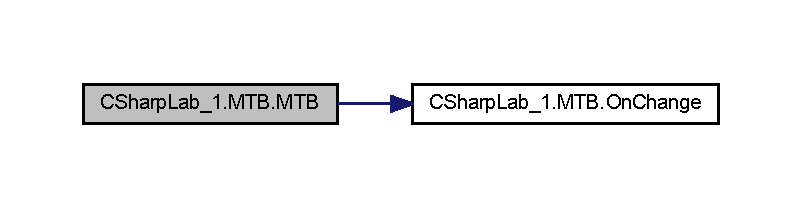
\includegraphics[width=350pt]{class_c_sharp_lab__1_1_1_m_t_b_a795c8d94ca1b20c77870728ae387d302_cgraph}
\end{center}
\end{figure}


\subsection{Member Function Documentation}
\hypertarget{class_c_sharp_lab__1_1_1_m_t_b_adabad767120ebeffbeba7beef05263ce}{}\label{class_c_sharp_lab__1_1_1_m_t_b_adabad767120ebeffbeba7beef05263ce} 
\index{C\+Sharp\+Lab\+\_\+1\+::\+M\+TB@{C\+Sharp\+Lab\+\_\+1\+::\+M\+TB}!Event\+Start@{Event\+Start}}
\index{Event\+Start@{Event\+Start}!C\+Sharp\+Lab\+\_\+1\+::\+M\+TB@{C\+Sharp\+Lab\+\_\+1\+::\+M\+TB}}
\subsubsection{\texorpdfstring{Event\+Start()}{EventStart()}}
{\footnotesize\ttfamily void C\+Sharp\+Lab\+\_\+1.\+M\+T\+B.\+Event\+Start (\begin{DoxyParamCaption}{ }\end{DoxyParamCaption})}



Обробник подій 

\hypertarget{class_c_sharp_lab__1_1_1_m_t_b_a0a6eccaa6ad4e983c7f3fa47d6b926a9}{}\label{class_c_sharp_lab__1_1_1_m_t_b_a0a6eccaa6ad4e983c7f3fa47d6b926a9} 
\index{C\+Sharp\+Lab\+\_\+1\+::\+M\+TB@{C\+Sharp\+Lab\+\_\+1\+::\+M\+TB}!Get\+Amount@{Get\+Amount}}
\index{Get\+Amount@{Get\+Amount}!C\+Sharp\+Lab\+\_\+1\+::\+M\+TB@{C\+Sharp\+Lab\+\_\+1\+::\+M\+TB}}
\subsubsection{\texorpdfstring{Get\+Amount()}{GetAmount()}}
{\footnotesize\ttfamily int C\+Sharp\+Lab\+\_\+1.\+M\+T\+B.\+Get\+Amount (\begin{DoxyParamCaption}{ }\end{DoxyParamCaption})}



Гетер 

\begin{DoxyReturn}{Returns}
Кількість обладнання
\end{DoxyReturn}
\hypertarget{class_c_sharp_lab__1_1_1_m_t_b_af571bf7359805b314bd1535dede971e2}{}\label{class_c_sharp_lab__1_1_1_m_t_b_af571bf7359805b314bd1535dede971e2} 
\index{C\+Sharp\+Lab\+\_\+1\+::\+M\+TB@{C\+Sharp\+Lab\+\_\+1\+::\+M\+TB}!On\+Change@{On\+Change}}
\index{On\+Change@{On\+Change}!C\+Sharp\+Lab\+\_\+1\+::\+M\+TB@{C\+Sharp\+Lab\+\_\+1\+::\+M\+TB}}
\subsubsection{\texorpdfstring{On\+Change()}{OnChange()}}
{\footnotesize\ttfamily delegate void C\+Sharp\+Lab\+\_\+1.\+M\+T\+B.\+On\+Change (\begin{DoxyParamCaption}{ }\end{DoxyParamCaption})}



Делегат 

Here is the caller graph for this function\+:
\nopagebreak
\begin{figure}[H]
\begin{center}
\leavevmode
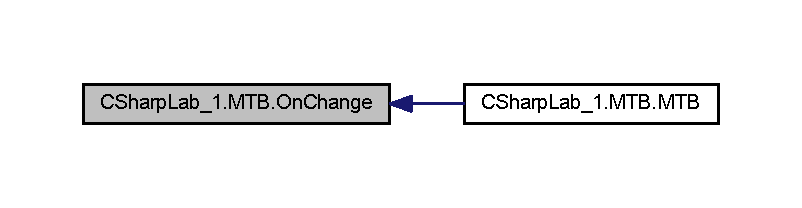
\includegraphics[width=350pt]{class_c_sharp_lab__1_1_1_m_t_b_af571bf7359805b314bd1535dede971e2_icgraph}
\end{center}
\end{figure}


\subsection{Event Documentation}
\hypertarget{class_c_sharp_lab__1_1_1_m_t_b_a7b0c9b5105656ce802a60a45128bde81}{}\label{class_c_sharp_lab__1_1_1_m_t_b_a7b0c9b5105656ce802a60a45128bde81} 
\index{C\+Sharp\+Lab\+\_\+1\+::\+M\+TB@{C\+Sharp\+Lab\+\_\+1\+::\+M\+TB}!Amortize@{Amortize}}
\index{Amortize@{Amortize}!C\+Sharp\+Lab\+\_\+1\+::\+M\+TB@{C\+Sharp\+Lab\+\_\+1\+::\+M\+TB}}
\subsubsection{\texorpdfstring{Amortize}{Amortize}}
{\footnotesize\ttfamily \hyperlink{class_c_sharp_lab__1_1_1_m_t_b_af571bf7359805b314bd1535dede971e2}{On\+Change} C\+Sharp\+Lab\+\_\+1.\+M\+T\+B.\+Amortize}



Подія списання 

\hypertarget{class_c_sharp_lab__1_1_1_m_t_b_ae07bfca3c3f690f17960215d7570d247}{}\label{class_c_sharp_lab__1_1_1_m_t_b_ae07bfca3c3f690f17960215d7570d247} 
\index{C\+Sharp\+Lab\+\_\+1\+::\+M\+TB@{C\+Sharp\+Lab\+\_\+1\+::\+M\+TB}!Bought@{Bought}}
\index{Bought@{Bought}!C\+Sharp\+Lab\+\_\+1\+::\+M\+TB@{C\+Sharp\+Lab\+\_\+1\+::\+M\+TB}}
\subsubsection{\texorpdfstring{Bought}{Bought}}
{\footnotesize\ttfamily \hyperlink{class_c_sharp_lab__1_1_1_m_t_b_af571bf7359805b314bd1535dede971e2}{On\+Change} C\+Sharp\+Lab\+\_\+1.\+M\+T\+B.\+Bought}



Подія закупівлі 

\hypertarget{class_c_sharp_lab__1_1_1_m_t_b_a98818a5eca5d6356b98673aa004532d9}{}\label{class_c_sharp_lab__1_1_1_m_t_b_a98818a5eca5d6356b98673aa004532d9} 
\index{C\+Sharp\+Lab\+\_\+1\+::\+M\+TB@{C\+Sharp\+Lab\+\_\+1\+::\+M\+TB}!Brouken@{Brouken}}
\index{Brouken@{Brouken}!C\+Sharp\+Lab\+\_\+1\+::\+M\+TB@{C\+Sharp\+Lab\+\_\+1\+::\+M\+TB}}
\subsubsection{\texorpdfstring{Brouken}{Brouken}}
{\footnotesize\ttfamily \hyperlink{class_c_sharp_lab__1_1_1_m_t_b_af571bf7359805b314bd1535dede971e2}{On\+Change} C\+Sharp\+Lab\+\_\+1.\+M\+T\+B.\+Brouken}



Подія поломки 



The documentation for this class was generated from the following file\+:\begin{DoxyCompactItemize}
\item 
M\+T\+B.\+cs\end{DoxyCompactItemize}

\hypertarget{class_c_sharp_lab__1_1_1_program}{}\section{C\+Sharp\+Lab\+\_\+1.\+Program Class Reference}
\label{class_c_sharp_lab__1_1_1_program}\index{C\+Sharp\+Lab\+\_\+1.\+Program@{C\+Sharp\+Lab\+\_\+1.\+Program}}


The documentation for this class was generated from the following file\+:\begin{DoxyCompactItemize}
\item 
Program.\+cs\end{DoxyCompactItemize}

%--- End generated contents ---

% Index
\backmatter
\newpage
\phantomsection
\clearemptydoublepage
\addcontentsline{toc}{chapter}{Index}
\printindex

\end{document}
